\documentclass[b5paper]{book}
\usepackage[spanish]{babel}
\usepackage[latin1]{inputenc}
\usepackage{graphicx}
\special{pdf: pagesize width 17.6cm height 25.1cm}


\usepackage{fancyhdr}
\pagestyle{fancy}
\lfoot[\fancyplain{}{\thepage}]     {\fancyplain{}{}}
\cfoot[\fancyplain{}{}]     {\fancyplain{}{}}
\rfoot[\fancyplain{}{}]     {\fancyplain{}{\thepage}}


\title{PFC:An�lisis}
\author{Javier Casas Velasco}
\date{No terminado}


%\voffset=-1.54cm


\evensidemargin=-0.54cm
\oddsidemargin=-1.04cm
\textwidth=14.1cm
\headwidth=14.1cm
%\usepackage[pdftex,
%        colorlinks=true,
%        urlcolor=rltblue,       % \href{...}{...} external (URL)
%        filecolor=rltgreen,     % \href{...} local file
%        linkcolor=rltred,       % \ref{...} and \pageref{...}
%        pdftitle={Untitled},
%        pdfauthor={Your Name},
%        pdfsubject={Just a test},
%        pdfkeywords={test, testing, testable stuff},
%        pdfproducer={pdfLaTeX},
%        pdfadjustspacing=1,
%        pagebackref,
%        pdfpagemode=None,
%        bookmarksopen=true]{hyperref}
%\usepackage{color}
%\definecolor{rltred}{rgb}{0.75,0,0}
%\definecolor{rltgreen}{rgb}{0,0.5,0}
%\definecolor{rltblue}{rgb}{0,0,0.75}


\begin{document}
%\maketitle
\chapter{Introducci�n}
El videojuego es uno de los �ltimos tipos de entretenimiento inventados. Heredando su legado de la imaginaci�n y la inform�tica, el videojuego es la especificaci�n en forma de programa inform�tico de lo que la mente del dise�ador pens� que ser�a divertido y entretenido.

\chapter{Propiedades del videojuego}
El videojuego tiene muchas propiedades, algunas heredadas de la inform�tica o el juego, y otras que aparecen en el desarrollo del mismo.
\section{Propiedades objetivas}
Con este nombre calificaremos las propiedades que son f�cilmente medibles.
\begin{itemize}
\item Coste de desarrollo \newline El videojuego, como programa inform�tico, tiene un coste que es lo que se gasta una empresa para desarrollarlo.
\item Calidad gr�fica \newline Define la calidad que tiene la parte visual del juego.
\item Calidad de sonido \newline Define la calidad que tiene la parte auditiva del juego.
\item Linealidad \newline Define la libertad que tiene el jugador dentro del juego para tomar decisiones.
\item Trama \newline Al igual que una pel�cula, la trama de un videojuego define una historia en la que el jugador participa, t�picamente como protagonista.
\item G�nero \newline El g�nero de un videojuego define el estilo de dificultades e interactividad.
\end{itemize}
\section{Propiedades subjetivas}
Con este nombre calificaremos las propiedades cuya medida sea dif�cil o imposible.
\begin{itemize}
\item Dificultad \newline
\item Adictividad \newline
\item Jugabilidad \newline
\item Diversi�n \newline
\item Inmersi�n \newline
\item Interactividad \newline

\end{itemize}
\chapter{G�neros del videojuego}
Al igual que hay distintos g�neros de pel�culas, pongamos por ejemplo, comedias, pel�culas b�licas, de esp�as o del oeste; tambi�n hay g�neros en el videojuego. El g�nero determina la interactividad y, a menudo, el argumento. A continuaci�n hay una lista de los g�neros m�s famosos del videojuego.
\begin{itemize}
\item FPS o First Person Shooters \newline
Juegos de disparos, donde el punto de vista es el que tendr�a el protagonista. El jugador juega dentro del papel de una persona envuelta en un mundo de armas de fuego en el que tiene que sobrevivir. Las capacidades necesarias en este tipo de juego suelen ser la capacidad de esconderse, la emboscada y la punter�a con las armas.
\item Estrategia \newline
Juegos en los que el jugador ve la acci�n pero no est� implicado directamente. T�picamente el jugador ve el mundo desde un punto de vista superior, de la misma manera que el jugador de ajedrez ve el tablero desde arriba. En estos juegos, el jugador env�a �rdenes a sus piezas, las unidades, que son las que deber�n luchar contra otras piezas para ganar la partida. Las capacidades necesarias en este tipo de juego suelen ser la organizaci�n, la planificaci�n y el conocimiento del enemigo.
\item Simuladores \newline
Juegos que simulan de una manera lo m�s realista posible situaciones del mundo real, o situaciones que podr�an darse en el mundo real. El jugador se ve envuelto en un entorno muy parecido a la realidad, en el que su habilidad determina el desenlace de la situaci�n. A menudo se simula el control de un veh�culo, t�picamente un avi�n. Las capacidades necesarias en este tipo de juego suelen ser las necesarias para la situaci�n real correspondiente.
\item Puzzles \newline

\end{itemize}

\chapter{Visi�n general}
Como ya se ha comentado, en este sistema pretendemos conseguir un mecanismo de aceleraci�n del desarrollo de un videojuego, ofreciendo para ello una parte del trabajo ya hecho. As� esa parte tan s�lo hay que retocarla y adaptarla al caso concreto. Por otra parte debe ser sencillo de manejar, con el fin de evitar que el coste de entrenar a los ingenieros para usarlo sea menor que el de desarrollar uno nuevo desde cero.

Por ello se busca que el sistema sea sencillo y extendible. Esto permitir� adaptarlo a los nuevos tiempos y a nuevas tecnolog�as. Esto implica que el sistema estar� desacoplado de bibliotecas concretas, con el fin de evitar que la desaparici�n de estas bibliotecas signifique el fin del sistema, y con la idea de poder adaptarlo a  bibliotecas nuevas.

Es evidente por lo indicado hasta ahora que este sistema est� orientado a desarrolladores.

En esta documentaci�n se distinguir� a dos tipos de usuarios:
\begin{itemize}
\item \textbf{El desarrollador} : Se le nombrar� normalmente como el usuario del producto, y es quien utiliza el sistema para desarrollar un videojuego.
\item \textbf{El jugador} : Es el usuario final, el que utiliza el videojuego desarrollado con el sistema que aqu� se expone.
\end{itemize}

\chapter{Requisitos funcionales}
\section{Introducci�n}
En este cap�tulo se describir� la funcionalidad de alto nivel del sistema.
\section{Requisitos del sistema en conjunto}
\begin{itemize}
\Requisito{1}{El sistema proporcionar� una ayuda al desarrollo de videojuegos.}{Imprescindible}{}
\Requisito{2}{El sistema proporcionar� un subsistema gr�fico listo para ser utilizado.}{Imprescindible}{}
\Requisito{3}{El sistema proporcionar� un subsistema de sonido listo para ser utilizado. En esta revisi�n no se incluye el desarrollo de dicho sistema.}{No implementado en esta revisi�n.}{}
\Requisito{4}{El sistema proporcionar� un subsistema de entrada listo para ser utilizado. En esta revisi�n no se incluye el desarrollo de dicho sistema.}{No implementado en esta revisi�n.}{}
\Requisito{5}{El sistema proporcionar� un esqueleto para facilitar la implementaci�n de la l�gica del juego.}{Imprescindible}{}
\Requisito{6}{El sistema proporcionar� el esqueleto t�pico de las aplicaciones interactivas.}{Imprescindible}{}
\end{itemize}

\section{Requisitos del subsistema gr�fico}
En esta secci�n nos referiremos al subsistema gr�fico como sistema gr�fico o motor gr�fico, para abreviar.

\begin{itemize}
\Requisito{2.1}{El motor gr�fico estar� orientado a las 3 dimensiones del espacio.}{Imprescindible}{}
\Requisito{2.2}{El motor gr�fico estar� organizado en torno al uso de pol�gonos como su estructura b�sica de representaci�n.}{Imprescindible}{}
	\begin{itemize}
	\Requisito{2.2.1}{Los pol�gonos soportar�n texturizado e iluminaci�n.}{Imprescindible}{}
	\Requisito{2.2.2}{El sistema proveer� un mecanismo para la importaci�n y carga de grandes grupos de pol�gonos (mallas).}{Imprescindible}{}
	\Requisito{2.2.3}{El motor gr�fico proveer� de una estructura b�sica para el manejo y procesamiento de mallas de pol�gonos.}{Imprescindible}{}
	\end{itemize}
\Requisito{2.3}{El motor gr�fico deber� ser f�cilmente desacoplable de la biblioteca gr�fica que se utilice.}{Imprescindible}{}
	\begin{itemize}
	\Requisito{2.3.1}{Inicialmente se utilizar� la biblioteca gr�fica OpenGL.}{Imprescindible}{}
	\end{itemize}
\Requisito{2.4}{El motor gr�fico tendr� disponibles entidades de alto nivel para su utilizaci�n.}{Imprescindible}{}
	\begin{itemize}
	\Requisito{2.4.1}{Una entidad de alto nivel ser� el objeto. Los objetos permitir�n manipular elementos de la escena como son c�maras y luces de una manera sencilla.}{Imprescindible}{}
	\Requisito{2.4.2}{Otra entidad de alto nivel ser� la pantalla. Las escenas agrupan objetos y se pintan en la pantalla, para que el jugador pueda verlas.}{Imprescindible}{}
	\end{itemize}
\Requisito{2.5}{El motor gr�fico estar� orientado a representar gr�ficos en tiempo real en la pantalla.}{Imprescindible}{}
\end{itemize}

%\section{Requisitos del subsistema de sonido}


%\section{Requisitos del subsistema de entrada}
%\begin{itemize}
%\Requisito{4.1}{El sistema proporcionar� un mecanismo para utilizar los dispositivos de entrada.}{Imprescindible}{}
%\Requisito{4.2}{El sistema simplificar� la utilizaci�n de los dispositivos de entrada.}{Imprescindible}{}
%	\begin{itemize}
%	\Requisito{4.2.1}{Existir� un tipo de dispositivo llamado binario, que en un determinado momento estar� o activado o desactivado.}{Imprescindible}{}
%	\Requisito{4.2.2}{Existir� un tipo de dispositivo llamado lineal, que en un determinado momento valdr� un valor en un intervalo.}{Imprescindible}{}
%	\Requisito{4.2.3}{Existir� un tipo de dispositivo llamado compuesto, y que ser� un agregado de otros dispositivos.}{Impresicindible}{}
%	\Requisito{4.2.4}{El sistema organizar� los dispositivos de entrada disponibles seg�n el esquema indicado anteriormente de dispositivos binarios, lineales y compuestos.}{Imprescindible}{}
%	\end{itemize}
%\end{itemize}


\section{Requisitos del esqueleto para la implementaci�n de la l�gica del juego}
\begin{itemize}
\Requisito{5.1}{El sistema proporcionar� un mecanismo para crear y procesar entidades concurrentes dentro del juego.}{Imprescindible}{}
\Requisito{5.2}{El sistema proporcionar� un mecanismo para el control eficiente y adecuado del tiempo dentro del juego.}{Alta}{}
\end{itemize}

\section{Requisitos del esqueleto de aplicaci�n interactiva}
\begin{itemize}
\Requisito{6.1}{El sistema proporcionar� un bucle principal.}{Imprescindible}{}
\Requisito{6.2}{El sistema estar� estructurado seg�n el modelo de bucle principal t�pico de aplicaci�n interactiva: 
	\begin{enumerate}
	\item Leer entrada
	\item Procesar informaci�n
	\item Representar resultados
	\item Ir a 1
	\end{enumerate} \ }{Imprescindible}{}
	
\end{itemize}

%\section{Requisitos del subsistema de entrada}
%A continuaci�n se enumeran los requisitos que tiene el sistema para aceptar entradas del jugador.
%\begin{enumerate}
%\item \ReqImprescindible{Interfaz de entrada}{El sistema debe proveer un subsistema capaz de leer entradas desde distinto hardware}{Ninguna}
%\item \ReqImprescindible{Teclado}{El sistema debe poder leer pulsaciones de teclas en el teclado en la forma ``pulsar tecla'' y ``soltar tecla'', con las limitaciones impuestas por el hardware}{Interfaz de entrada}
%\item \ReqImprescindible{Rat�n}{El sistema debe poder leer informaci�n disponible de uno o varios ratones o dispositivos equivalentes (trackball) en la forma ``pulsar bot�n'', ``soltar bot�n'', ``desplazamiento del rat�n'' y posiblemente ``lectura de ejes alternativos'' en el caso de que el rat�n disponga de ruletas u otros dispositivos}{Interfaz de entrada}
%\item \ReqImprescindible{Joypad}{El sistema debe poder leer informaci�n disponible de mandos de juegos en la forma ``posici�n de la palanca/cruceta'', ``pulsar bot�n'', ``soltar bot�n'' y ``posici�n de ejes alternativos''}{Interfaz de entrada}
%\item \ReqAlta{Otros dispositivos}{El sistema debe proveer mecanismos para la extensi�n y el soporte de nuevos mandos de entrada que aparezcan}{Intefaz de entrada}
%\item \ReqAlta{Unificaci�n del acceso}{El acceso a la informaci�n prove�da por los dispositivos debe ser lo m�s uniforme posible}{Ninguna}
%\item \ReqAlta{Demoras en el acceso}{El sistema debe implementar los mecanismos de acceso al hardware de entrada de una manera tal que la informaci�n se transfiera desde el hardware hasta la l�gica del juego con un retardo m�nimo}{Ninguna}
%\item \ReqAlta{Binding}{El enlace de datos entre el hardware y la l�gica del juego debe ser configurable en tiempo de ejecuci�n, con el fin garantizar la posibilidad de reconfigurar los controles en cualquier momento}{Ninguno}
%\end{enumerate}

%\section{Requisitos del subsistema de sonido}
%A continuaci�n se enumeran los requisitos dedicados a la parte sonora del sistema.
%
%\begin{enumerate}
%\item \ReqImprescindible{Sistema de sonido}{El sistema debe proveer un subsistema que pueda manejar y enviar sonidos a la tarjeta de sonido del sistema}{Ninguna}
%\end{enumerate}

%Con el fin de clasificar mejor estos requisitos se han agrupado en dos grupos: efectos de sonido y m�sica.

%\subsection{Efectos de sonido}
%\begin{enumerate}
%\item \ReqImprescindible{Efectos de sonido}{El sistema debe proveer un mecanismo para reproducir sonidos}{Sistema de sonido}
%\item \ReqImprescindible{Reproducci�n m�ltiple}{Los efectos de sonido se podr�n comenzar a reproducir a petici�n de la l�gica del juego en cualquier momento, pudiendo superponerse unos a otros}{Efectos de sonido}
%\item \ReqImprescindible{Control de volumen}{Debe proveerse un mecanismo que permita controlar el volumen de reproducci�n de un determinado efecto de sonido, con independencia de los dem�s efectos de sonido (inclu�das copias de �l mismo)}{Efectos de sonido}
%\item \ReqMedia{Velocidad de reproducci�n}{Debe existir un mecanismo que permita controlar la velocidad de reproducci�n de un efecto de sonido, con independencia de los dem�s efectos de sonido (inclu�das copias de �l mismo)}{Efectos de sonido}
%\item \ReqAlta{Est�reo o cuadraf�nico}{Debe haber un mecanismo que permita posicionar un sonido en el espacio con el fin de que suene adecuadamente en sistemas de altavoces en est�reo o cuadraf�nicos}{Efectos de sonido}
%\item \ReqAlta{Formatos est�ndar}{El sistema debe soportar la carga de efectos de sonido en la forma de sonidos con formato est�ndar}{Efectos de sonido}
%\end{enumerate}

%\subsection{M�sica}
%\begin{enumerate}
%\item \ReqImprescindible{M�sica}{El sistema debe proveer un mecanismo para reproducir m�sica}{Sistema de sonido}
%\item \ReqImprescindible{Control de reproducci�n}{El sistema de m�sica debe proveer un mecanismo para poder avanzar, parar, pausar, controlar el volumen o reproducir m�sica, siguiendo los conceptos que esto representar�a en un reproductor de CD}{M�sica}
%\item \ReqMedia{Reproducci�n m�ltiple}{El sistema debe poder reproducir varias m�sicas simult�neamente, y controlar cada una por separado de la manera que en el requisito \emph{Control de reproducci�n} se especifica }{M�sica}
%\item \ReqAlta{Carga diferida}{Debido a que el sistema no puede almacenar en memoria RAM gran cantidad de m�sica descomprimida, debe existir un mecanismo que cargue la m�sica en tiempo real de disco, a medida que se necesite}{M�sica}
%\item \ReqAlta{Formatos est�ndar}{El sistema debe soportar la carga de m�sica desde formatos est�ndar. Recomendados: MPEG Audio Layer-3 (MP3) y Ogg Vorbis (OGG)}{M�sica}
%\end{enumerate}


\chapter{Requisitos no funcionales}
\section{Facilidad de uso}
\section{Confiabilidad}
\begin{itemize}
\Requisito{N1}{El sistema debe estar implementado bajo unos modelos y unas pr�cticas que minimicen la necesidad de correcci�n de errores de implementaci�n en el futuro.}{Alta}{}
\end{itemize}

\section{Perfomance}
\begin{itemize}
\Requisito{N2}{El sistema debe ser r�pido en tiempo de ejecuci�n, y por tanto debe estar optimizado para funcionar lo m�s r�pido posible.}{Imprescindible}{}
\end{itemize}

\section{Restricciones de dise�o}
\begin{itemize}
\Requisito{N3}{El sistema debe estar dise�ado con la idea de poder portarlo con facilidad a otras arquitecturas o sistemas operativos.}{Imprescindible}{}
\end{itemize}

\section{Seguridad}
\begin{itemize}
\Requisito{N4}{El sistema debe ser resistente a ataques por parte de piratas inform�ticos ya sea local o remotamente.}{Medio}{}
\end{itemize}

\section{Documentaci�n de usuario y sistemas de ayuda}
\begin{itemize}
\Requisito{N5}{El sistema debe disponer de una documentaci�n de dise�o del mismo.}{Imprescindible}{}
\Requisito{N6}{El sistema debe disponer de una gu�a de funciones, objetos y clases que permitan a un desarrollador utilizarlo con facilidad.}{Imprescindible}{}
\end{itemize}

\section{Interfaces}
\subsection{Interfaces de usuario}
\begin{itemize}
\Requisito{N7.1}{El sistema debe proporcionar un interfaz para la visualizaci�n, audici�n e interactividad con el sistema.}{Imprescindible}{}
\end{itemize}
%\subsection{Interfaces Hardware}
\subsection{Interfaces Software}
\begin{itemize}
\Requisito{N7.2}{El sistema debe proporcionar un interfaz software que permita utilizarlo para desarrollar programas, es decir, debe ser integrable a un compilador y un generador de c�digo m�quina.}{Imprescindible}{}
\end{itemize}
%\subsection{Interfaces de comunicaci�n}


\newcommand{\flecha}[0]{-\textgreater\ }

\chapter{Modelos del sistema}
\section{Sistema gr�fico}
Se propone dividir el motor gr�fico en varios niveles, con el fin de simplificar las relaciones y reducir la dependencia. Por ello se proponen tres niveles:
\begin{itemize}
\item \textbf{Nivel de geometr�a} : Trata con v�rtices, pol�gonos y mallas
\item \textbf{Nivel de objetos} : Trata con los objetos que componen una escena, c�maras y luces
\item \textbf{Nivel de dibujado} : Trata de c�mo manejar las escenas que componen la imagen final que se muestra en pantalla
\end{itemize}



\subsection{Nivel de geometr�a}
Este nivel organiza el almacenamiento y proceso de las mallas de pol�gonos y los elementos que las componen. Est� organizado como clases de almacenamiento de datos (clases entidad) ya que apenas hay procesamiento en este subsistema, al menos respecto a la parte que ser� implementada en esta revisi�n.

\subsection{Nivel de objetos}
Este nivel organiza el procesamiento de las entidades que componen una escena, trat�ndolas como entidades indivisibles. Incluye el caso de uso \emph{emparentar}, que se encarga de describir c�mo unos objetos pueden depender de otros geom�tricamente hablando.

\subsection{Nivel de dibujado}
Este nivel se ha organizado para poder controlar varias pantallas con distintos sistemas e im�genes en cada una.

\section{Motor de procesos}
Este subsistema se encarga de proporcionar un esqueleto para la l�gica del juego. Para ello propone dividir dicha l�gica en peque�os elementos que se ejecutan concurrentemente como los procesos en un sistema operativo. Incluye los casos de uso \emph{ejecutar\_procesos}, que se encarga de dar tiempo de CPU a cada proceso; y \emph{cambiar\_prioridad}, que se encarga de decidir el orden en que se ejecutar�n los procesos.

\chapter{Escenarios}
\section{Sistema gr�fico}


\chapter{Modelo de casos de uso}
En este cap�tulo se describir�n los casos de uso principales.

\section{Descripciones generales de actores}
\begin{itemize}
\item \textbf{Desarrollador} : El desarrollador utiliza el sistema para desarrollar su videojuego.
\item \textbf{Usuario} : El usuario en un caso de uso suele ser el propio software a�adido por el desarrollador para utilizar el framework. A menudo tambi�n ser� cualquier otra parte del sistema que dependa de la que se est� describiendo actualmente. En esos casos en la descripci�n del caso de uso se indicar� qui�n es un buen candidato a usar el sistema.
\item \textbf{Main Loop} : A menudo, el bucle principal de la aplicaci�n iniciar� un caso de uso.
\item \textbf{Proceso} : Muchas veces, parte de la l�gica del juego, expresada como procesos, iniciar� un caso de uso.
\end{itemize}
\section{Diagrama de modelo de casos de uso}

\section{General: bucle principal}
El modelo de ejecuci�n general del programa. Est� basado en el modelo de ejecuci�n de un programa interactivo, adaptado para este sistema.
\subsection{Flujo b�sico}
\begin{enumerate}
\item El sistema se inicializa.
\item Mientras deba continuar la ejecuci�n del sistema:
	\begin{enumerate}
	\item El jugador genera eventos de entrada si desea.
	\item Si hay eventos de entrada:
		\begin{enumerate}
		\item El sistema procesa los eventos de entrada.
		\end{enumerate}
	\item El sistema procesa la informaci�n del juego.
	\item El sistema muestra el resultado del procesamiento.
	\item El jugador ve el resultado de sus acciones.
	\end{enumerate}
\item El sistema libera recursos y finaliza su ejecuci�n.
\end{enumerate}
\subsection{Requisitos especiales}
\subsection{Precondiciones}
\subsection{Postcondiciones}
\subsection{Puntos de extensi�n}
\subsection{Relaciones}
\subsection{Otros diagramas}


\section{Objetos: emparentar objeto}
Cambia de padre a un objeto. Sirve para desplazar ese objeto por el �rbol de objetos.
\subsection{Flujo b�sico}
\begin{enumerate}
\item El usuario ordena al objeto cambiar de padre, y especifica un nuevo padre.
\item Si el objeto ten�a otro padre anteriormente:
	\begin{enumerate}
	\item El objeto se libera de la dependencia con su padre anterior.
	\end{enumerate}
\item El objeto establece una dependencia con su nuevo padre.
\end{enumerate}

\subsection{Requisitos especiales}
\subsection{Precondiciones}
\subsection{Postcondiciones}
\subsection{Puntos de extensi�n}
\subsection{Relaciones}
\subsection{Otros diagramas}

\chapter{Modelos Objeto}
\section{Nivel de geometr�a}
Este nivel se ha propuesto principalmente como un mecanismo para almacenar y procesar geometr�a, y ha sido organizado seg�n el modelo de datos de almacenamiento de geometr�a. En los sistemas m�s sencillos, la geometr�a a nivel de pol�gono tan solo debe ser consultada para pintarla en pantalla. Por ello no se contemplan operaciones complejas y raras, como pueden ser deformaciones din�micas y operaciones CSG (Geometr�a S�lida Constructiva).

\begin{figure}[htp]
\centering
%\includegraphics[width=14cm]{analisis/propuesto/modelos_objeto/geometria/clases.eps}
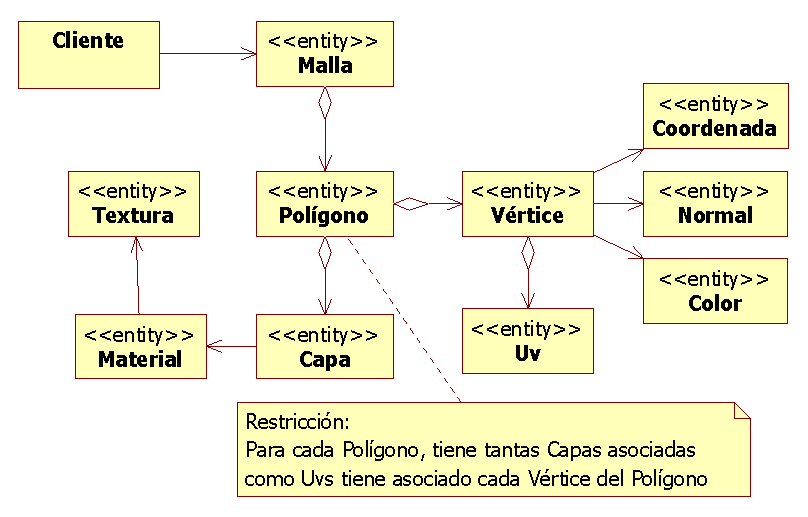
\includegraphics[width=14cm]{diagramas/analisis/geometria-clases.eps}
\caption{Diagrama de clases de an�lisis del nivel de Geometr�a}
\end{figure}


A�n as�, este es el modelo abstracto, y puede ser extendido para soportar otras operaciones.
A continuaci�n se describir� la utilidad de cada clase:

\subsection{Coordenada}
Almacena una coordenada en el espacio 3D.
\begin{itemize}
\item \textbf{Responsabilidades:}
	\begin{itemize}
	\item Almacenar una coordenada del espacio.
	\end{itemize}
\item \textbf{Relaciones:}
	\begin{itemize}
	\item -valor : vector3 \newline
		Vector con las coordenadas almacenadas.
	\end{itemize}
\item \textbf{M�todos:}
	\begin{itemize}
	\item \emph{+creaci�n}(v:vector3) : coordenada \newline
		Hace una coordenada nueva con valor v.
	\item +valor() : vector3 \newline
		Vector con las coordenadas almacenadas.
	\end{itemize}
\end{itemize}

\subsection{Normal}
Almacena una direcci�n normal.
\begin{itemize}
\item \textbf{Responsabilidades:}
	\begin{itemize}
	\item Almacenar una direcci�n normal.
	\item Mantener dicha direcci�n normal unitaria (vector de longitud 1).
	\end{itemize}
\item \textbf{Relaciones:}
	\begin{itemize}
	\item -valor : vector3 \newline
		Vector con la normal almacenada.
	\end{itemize}
\item \textbf{M�todos:}
	\begin{itemize}
	\item \emph{+creaci�n}(v:vector3) : normal \newline
		Hace una normal nueva con valor v.
	\item +valor() : vector3 \newline
		Vector con la normal.
	\end{itemize}
\end{itemize}

\subsection{Color}
Almacena un color. El color se almacena en formato RGBA, esto es, las componentes de los vectores representan los colores en orden Rojo, Verde, Azul, Alfa, donde Alfa es el valor de transparencia. Los valores pueden variar en el intervalo [0..1], donde 0 es intensidad nula y 1 es intensidad m�xima. Para el valor de Alfa, 1 significa completamente opaco y 0 significa completamente transparente.
\begin{itemize}
\item \textbf{Responsabilidades:}
	\begin{itemize}
	\item Almacenar un color.
	\item Almacenar un valor de transparencia.
	\end{itemize}
\item \textbf{Relaciones:}
	\begin{itemize}
	\item -valor : vector4 \newline
		Vector con el color en formato RGBA.
	\end{itemize}
\item \textbf{M�todos:}
	\begin{itemize}
	\item \emph{+creaci�n}(v:vector4) : color \newline
		Hace un color nuevo con valor v.
	\item +valor() : vector4 \newline
		Vector con el color en formato RGBA.
	\end{itemize}
\end{itemize}

\subsection{UV}
Almacena una coordenada UV o de texturizado.

Restricci�n: Para cada v�rtice de un determinado pol�gono debe haber tantas coordenadas UV como capas tenga el pol�gono.

\begin{itemize}
\item \textbf{Responsabilidades:}
	\begin{itemize}
	\item Almacenar una coordenada de texturizado.
	\end{itemize}
\item \textbf{Relaciones:}
	\begin{itemize}
	\item -valor : vector2 \newline
		Vector con la coordenada UV.
	\end{itemize}
\item \textbf{M�todos:}
	\begin{itemize}
	\item \emph{+creaci�n}(v:vector2) : UV \newline
		Hace una UV nueva con valor v.
	\item +valor() : vector2 \newline
		Vector con la coordenada UV.
	\end{itemize}
\end{itemize}

\subsection{Material}
Almacena el material del que est� compuesta la suerficie de un pol�gono.
\begin{itemize}
\item \textbf{Responsabilidades:}
	\begin{itemize}
	\item Almacenar informaci�n de un material.
	\end{itemize}
\item \textbf{Relaciones:}
	\begin{itemize}
	\item -textura : textura \newline
		El mapa de bits que utiliza de textura
	\end{itemize}
\item \textbf{M�todos:}
	\begin{itemize}
	\item \emph{+creaci�n}(t:textura) : material \newline
		Hace un material nuevo con la textura t.
	\item +textura() : textura \newline
		El mapa de bits que utiliza de textura.
	\end{itemize}
\end{itemize}

\subsection{V�rtice}
Almacena un v�rtice de un pol�gono.
\begin{itemize}
\item \textbf{Responsabilidades:}
	\begin{itemize}
	\item Almacenar un v�rtice, con sus coordenadas, su posici�n de texturizado y la direcci�n normal de la superficie en ese punto.
	\end{itemize}
\item \textbf{Relaciones:}
	\begin{itemize}
	\item -coordenada : coordenada \newline
		La posici�n del v�rtice dentro del espacio.
	\item -normal : normal \newline
		La direcci�n normal del v�rtice.
	\item -color : color \newline
		El color del v�rtice.
	\item -uvs : colecci�n ordenada de UV \newline
		Las coordenadas UV de texturizado del v�rtice.
	\end{itemize}
\item \textbf{M�todos:}
	\begin{itemize}
	\item \emph{+creaci�n}(c:coordenada, n:normal, co:color, uvs:colecci�n ordenada de uv) : vertice \newline
		Hace un nuevo v�rtice con las caracter�sticas indicadas.
	\item +coordenada() : coordenada \newline
		La posici�n del v�rtice dentro del espacio.
	\item +normal() : normal \newline
		La direcci�n normal del v�rtice.
	\item +color() : color \newline
		El color del v�rtice.
	\item +uv(n:entero) : UV \newline
		Las coordenadas UV de texturizado del v�rtice, referidas a la capa n.
	\end{itemize}
\end{itemize}

\subsection{Capa}
Almacena la informaci�n referida a una capa que se aplica a un pol�gono.
\begin{itemize}
\item \textbf{Responsabilidades:}
	\begin{itemize}
	\item Almacenar informaci�n sobre una capa de pintado que se aplica sobre un conjunto de pol�gonos.
	\end{itemize}
\item \textbf{Relaciones:}
	\begin{itemize}
	\item -material : material \newline
		El material asociado a la capa.
	\end{itemize}
\item \textbf{M�todos:}
	\begin{itemize}
	\item \emph{+creaci�n}(m:material) : capa \newline
		Hace una nueva capa con material m.
	\item +material() : material \newline
		El material asociado a la capa.
	\end{itemize}
\end{itemize}

\subsection{Pol�gono}
Almacena la informaci�n de un pol�gono.

Restricci�n: Para cada v�rtice de un pol�gono debe haber tantas coordenadas UV como capas tenga el pol�gono.


\begin{itemize}
\item \textbf{Responsabilidades:}
	\begin{itemize}
	\item Almacenar los v�rtices y las capas de material de un pol�gono.
	\end{itemize}
\item \textbf{Relaciones:}
	\begin{itemize}
	\item -v�rtices : colecci�n ordenada de v�rtice \newline
		Los v�rtices del pol�gono.
	\item -capas : colecci�n ordenada de capa \newline
		Las capas de pintado que se aplican al pol�gono.
	\end{itemize}
\item \textbf{M�todos:}
	\begin{itemize}
	\item \emph{+creaci�n}(v:colecci�n ordenada de v�rtice, c:colecci�n ordenada de capa) : pol�gono \newline
		Hace un nuevo pol�gono con v�rtices v y capas c.
	\item +v�rtice(n:entero) : v�rtice \newline
		El n-�simo v�rtice.
	\item +capa(n:entero) : capa \newline
		La n-�sima capa.
	\end{itemize}
\end{itemize}

\subsection{Malla}
Almacena una malla de pol�gonos.
\begin{itemize}
\item \textbf{Responsabilidades:}
	\begin{itemize}
	\item Almacenar una malla de pol�gonos.
	\end{itemize}
\item \textbf{Relaciones:}
	\begin{itemize}
	\item -pol�gonos : colecci�n de pol�gono \newline
		Los pol�gonos de la malla.
	\end{itemize}
\item \textbf{M�todos:}
	\begin{itemize}
	\item \emph{+creaci�n}(p:colecci�n de pol�gono) : malla \newline
		Hace una nueva malla con los pol�gonos p.
	\item +pol�gonos() : colecci�n de pol�gono \newline
		Los pol�gonos de la malla.
	\end{itemize}
\end{itemize}



\section{Nivel de objetos}
Este nivel se ha propuesto con el fin de almacenar y ordenar adecuadamente los objetos. Por ello se propone organizarlos en forma de �rbol, donde la ra�z sea el punto de control y acceso del �rbol entero. Adem�s se utiliza esto para dar un significado extra a los objetos. La transformada de un objeto utiliza como origen de coordenadas las del objeto inmediatamente superior en el �rbol, que a su vez utiliza las del objeto superior, etc. Esto es cierto para todos los objetos excepto el objeto origen, que representa el origen de coordenadas del espacio. Esta caracter�stica permite implementar la capacidad de \emph{pegar} unos objetos a otros. El objeto \emph{pegado} pasar�a a ser descendiente del objeto al que ha sido pegado, y as�, al ejercer una transformada sobre el objeto padre el objeto pegado le seguir�a, \emph{pegado} a sus coordenadas locales.

\begin{figure}[htp]
\centering
%\includegraphics[width=14cm]{analisis/propuesto/modelos_objeto/objetos/clases.eps}
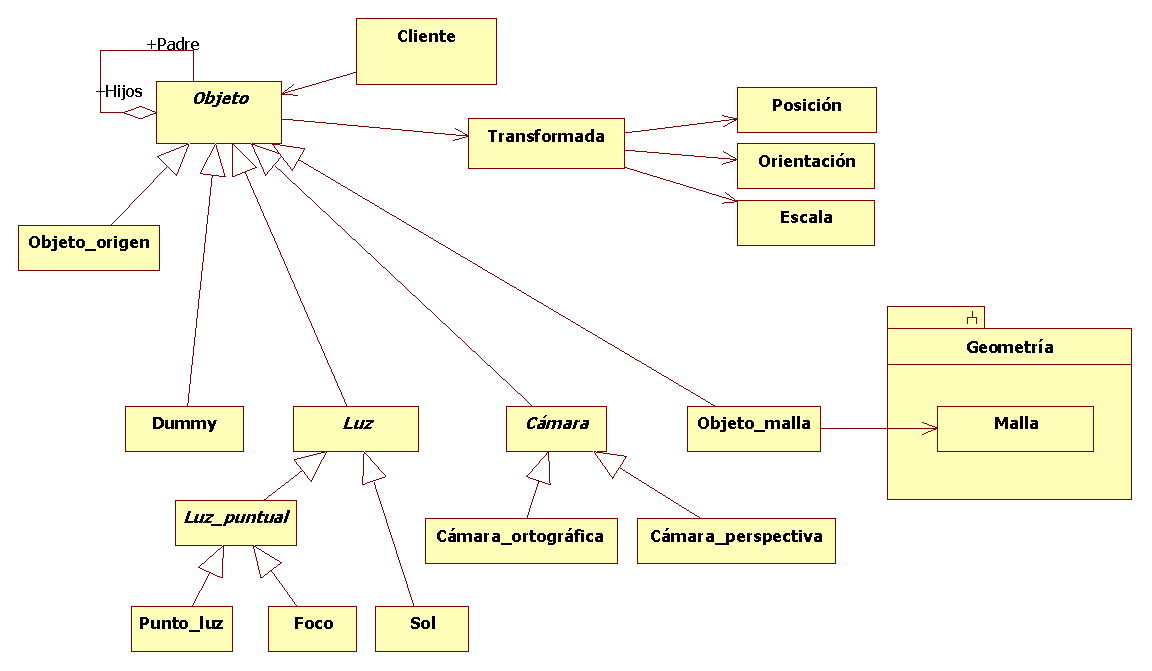
\includegraphics[width=14cm]{diagramas/analisis/objetos-clases.eps}

\caption{Diagrama de clases de an�lisis del nivel de Objetos}
\end{figure}


A continuaci�n se describe la utilidad de cada clase:

\subsection{Posici�n}
Almacena la indicaci�n de un lugar en el espacio.
\begin{itemize}
\item \textbf{Responsabilidades:}
	\begin{itemize}
	\item Almacenar una coordenada relativa en el espacio 3D.
	\item Proveer mecanismos para manipular esa coordenada.
	\end{itemize}
\item \textbf{Relaciones:}
	\begin{itemize}
	\item -coordenadas : vector3 \newline
		Coordenadas indicando la posici�n.
	\end{itemize}
\item \textbf{M�todos:}
	\begin{itemize}
	\item \emph{+creaci�n}() : posici�n \newline
		Hace una nueva posici�n situada en el origen relativo (coordenadas 0,0,0).
	\item +coordenadas() : vector3 \newline
		Las coordenadas que indican la posici�n.
	\item +mover(desplazamiento:vector3)\newline
		Mueve la posici�n la cantidad indicada.
	\item +establecer\_posici�n(p:vector3)\newline
		Sit�a la posici�n en el lugar indicado.
	\end{itemize}
\end{itemize}

\subsection{Orientaci�n}
Almacena una rotaci�n en el espacio. Hay que remarcar que la orientaci�n se puede especificar mediante dos vectores: uno que indica a d�nde apunta y otro que indica la vertical. Como vectores originales se propone (1,0,0) para la direcci�n de apunte y (0,1,0) para la vertical de un objeto que no ha sido rotado. No hay m�todos para rotaciones de Euler, pero se recuerda que estas se pueden obtener mediante una sucesi�n de tres rotaciones alrededor de los ejes xyz o zyx.
\begin{itemize}
\item \textbf{Responsabilidades:}
	\begin{itemize}
	\item Almacenar una rotaci�n en el espacio 3D.
	\item Proveer mecanismos para manipular esa rotaci�n.
	\end{itemize}
\item \textbf{Relaciones:}
	\begin{itemize}
	\item -valor : cuaterni�n \newline
		Cuaterni�n con la rotaci�n.
	\end{itemize}
\item \textbf{M�todos:}
	\begin{itemize}
	\item \emph{+creaci�n}() : orientaci�n \newline
		Hace una nueva orientaci�n nula (sin orientaci�n inicial).
	\item +rotar(v:vector3, angulo:float)\newline
		Rota la orientaci�n alrededor del vector especificado el �ngulo especificado (en grados).
	\item +establecer\_rotaci�n(v:vector3, angulo:float) \newline
		Modifica la orientaci�n para que tenga las caracter�sticas indicadas.
	\item +extraer\_rotaci�n() : (v:vector3, angulo:float) \newline
		Devuelve la orientaci�n como una �nica rotaci�n.
	\item +frontal() : vector3 \newline
		Devuelve la direcci�n a la que apunta la orientaci�n.
	\item +vertical() : vector3 \newline
		Devuelve la direcci�n vertical de la orientaci�n.
	\item +rotar\_vector(vector3) : vector3 \newline
		Aplica la orientaci�n al vector indicado.
	\end{itemize}
\end{itemize}

\subsection{Escala}
Almacena las dimensiones de forma relativa. Es decir, para un objeto, las dimensiones (1,1,1) corresponden a su tama�o original, mientras que (10,10,10) corresponder�a a un objeto 10 veces m�s grande en cada una de sus dimensiones. Se soportan dimensiones negativas, que significan que el objeto est� reflejado en el eje indicado. Tambi�n se soportan dimensiones nulas, que significan que el objeto est� proyectado sobre un subespacio de dimensi�n inferior. Esto debe ser tenido en cuenta por la implementaci�n concreta bajo un API concreto del motor gr�fico.
\begin{itemize}
\item \textbf{Responsabilidades:}
	\begin{itemize}
	\item Almacenar una definici�n de escala relativa en el espacio 3D.
	\item Proveer mecanismos para manipular esa definici�n de escala.
	\end{itemize}
\item \textbf{Relaciones:}
	\begin{itemize}
	\item -valor : vector3 \newline
		Vector con las tres dimensiones.
	\end{itemize}
\item \textbf{M�todos:}
	\begin{itemize}
	\item \emph{+creaci�n}() : escala \newline
		Hace una nueva escala con tama�o original (1,1,1).
	\item +escalar(vector3) \newline
		Multiplica el vector escala por el indicado, elemento a elemento y almacena el resultado.
	\item +establecer\_escala(vector3)\newline
		Modifica la escala para que tenga las caracter�sticas indicadas.
	\item +escala() : vector3 \newline
		Devuelve un vector con las tres componentes de la escala.
	\end{itemize}
\end{itemize}

\subsection{Transformada}
Almacena una transformada de un objeto. S�lo se almacenan la posici�n, orientaci�n y escala del objeto. Como se indic� antes, estas transformadas se almacenan relativamente respecto al objeto padre.
\begin{itemize}
\item \textbf{Responsabilidades:}
	\begin{itemize}
	\item Almacenar una definici�n de transformada relativa en el espacio 3D.
	\item La transformada debe soportar desplazamientos, rotaciones y escalas.
	\item Proveer mecanismos para manipular esa transformada.
	\end{itemize}
\item \textbf{Relaciones:}
	\begin{itemize}
	\item -posici�n : posici�n \newline
	\item -orientaci�n : orientaci�n \newline
	\item -escala : escala \newline
	\end{itemize}
\item \textbf{M�todos:}
	\begin{itemize}
	\item \emph{+creaci�n}() : transformada \newline
		Hace una nueva transformada. Esta transformada tiene las siguientes caracter�sticas:
		\begin{itemize}
		\item Posici�n: (0,0,0)
		\item Orientaci�n: Vector(1,0,0), �ngulo 0�
		\item Escala: (1,1,1)
		\end{itemize}
	\item +posici�n() : posici�n \newline
		La posici�n.
	\item +orientaci�n() : orientaci�n \newline
		La orientaci�n.
	\item +escala() : escala \newline
		La escala.
	\end{itemize}
\end{itemize}

\subsection{Objeto}
Almacena un objeto en el espacio. Esta clase es el modelo abstracto para acceder al �rbol de objetos que representa una escena, y de ella heredan los tipos concretos de objeto que se describir�n.
\begin{itemize}
\item \textbf{Responsabilidades:}
	\begin{itemize}
	\item Almacenar y organizar un objeto en el espacio.
	\item Proveer un mecanismo para la organizaci�n de objetos en forma de �rbol.
	\end{itemize}
\item \textbf{Relaciones:}
	\begin{itemize}
	\item \#padre : objeto opcional \newline
		El objeto inmediatamente superior en el �rbol de objetos (si est� metido en un �rbol de objetos).
	\item \#hijos : colecci�n de objeto \newline
		Los objetos que tienen a este objeto de padre.
	\item \#transformada : transformada \newline
		La transformada de este objeto.
	\end{itemize}
%\item \textbf{Atributos:}
%	\begin{itemize}
%	\end{itemize}
\item \textbf{M�todos:}
	\begin{itemize}
	\item \emph{+creaci�n}() : objeto \newline
		Crea el objeto nuevo e inicializa la tranformada.
	\item +padre() : objeto\newline
		El padre del objeto.
	\item \#set\_padre(objeto opcional)\newline
		Cambia el atributo \emph{padre}
	\item +hijos() : colecci�n de objeto\newline
		Los objetos hijo.
	\item \#set\_hijos(colecci�n de objeto)\newline
		Cambia el atributo \emph{hijos}
	\item +establecer\_padre(objeto)\newline
		Hace que el objeto indicado pase a ser el padre de este objeto, y este objeto pase a ser hijo del objeto indicado. Elimina otras dependencias con otros objetos si existieran.
	\item +origen() : objeto \newline
		El objeto origen del que depende el �rbol donde est� situado este objeto.
	\item +transformada() : transformada \newline
		Devuelve la transformada del objeto.
	\item +transformada\_final() : transformada \newline
		Computa la transformada desde el origen hasta el objeto actual, obteniendo una transformada que ser�a el resultado de aplicar cada una de las transformadas que afectan al objeto en orden.
	\end{itemize}
\end{itemize}

\subsection{Objeto\_origen}
Almacena el origen de coordenadas del espacio como objeto. Est� pensado para ser la ra�z del �rbol de objetos. Ya que todos los objetos dependen posicionalmente de �ste no tiene sentido modificar su transformada (todos los objetos, incluida la c�mara se ver�an afectados igual, y la escena no cambiar�a desde el punto de vista del observador).
\begin{itemize}
\item \textbf{Responsabilidades:}
	\begin{itemize}
	\item Proveer una ra�z para el �rbol de objetos.
	\end{itemize}
\item \textbf{Relaciones:}
	\begin{itemize}
	\item Es una especificaci�n de Objeto. \newline
		Es un tipo de objeto pensado para ser la ra�z del �rbol de objetos.
	\end{itemize}
\item \textbf{M�todos:}
	\begin{itemize}
	\item \emph{+creaci�n}() : objeto\_origen \newline
		Crea un objeto\_origen nuevo.
	\end{itemize}
\end{itemize}

\subsection{Dummy}
El dummy es un objeto nulo, que no afecta a la representaci�n en la pantalla. Sin embargo, puede ser utilizado para pegarle otros objetos y manipularlos en conjunto a trav�s de �ste.
\begin{itemize}
\item \textbf{Responsabilidades:}
	\begin{itemize}
	\item Proveer un objeto que no afecte a la representaci�n en la pantalla, pero pueda ser utilizado como punto de apoyo.
	\end{itemize}
\item \textbf{Relaciones:}
	\begin{itemize}
	\item Es una especificaci�n de Objeto. \newline
		Es un tipo de objeto pensado para ser la ra�z de sub-�rboles de objetos.
	\end{itemize}
\item \textbf{M�todos:}
	\begin{itemize}
	\item \emph{+creaci�n}() : dummy \newline
		Crea un dummy nuevo.
	\end{itemize}
\end{itemize}

\subsection{Luz}
Representa una fuente de luz que ilumina la escena. Tiene varias especializaciones que se especifican m�s adelante. Cabe resaltar que el color tambi�n especifica la \emph{cantidad} de luz. As�, una luz de color (1.0, 1.0, 1.0) es blanca de intensidad m�xima, mientras que una luz de color (0.5, 0.5, 0.5) tambi�n es blanca, pero de intensidad media. Una luz \emph{apagada} (que realmente no emite luz) tendr�a un color (0.0, 0.0, 0.0). La luz se divide en dos partes: difusa y especular. La parte difusa se refleja uniformemente en todas las direcciones. En cambio, la parte especular se refleja preferentemente en direcciones concretas, de una manera similar a como la luz se refleja en un espejo o una superficie pulida.
\begin{itemize}
\item \textbf{Responsabilidades:}
	\begin{itemize}
	\item Proveer un objeto que represente una fuente de luz.
	\end{itemize}
\item \textbf{Relaciones:}
	\begin{itemize}
	\item Es una especificaci�n de Objeto. \newline
		Es un tipo de objeto que representa una fuente de luz.
	\item \#color\_difuso : color \newline
		El color de la parte difusa de la luz
	\item \#color\_especular : color \newline
		El color de la parte especular de la luz
	\end{itemize}
\item \textbf{M�todos:}
	\begin{itemize}
	\item \emph{+creaci�n}() : luz \newline
		Inicializa la luz a valores por defecto. Estos son:
		\begin{itemize}
		\item Color difuso : (1.0,1.0,1.0)
		\item Color especular : (0.0,0.0,0.0)
		\end{itemize}
	\item +color\_difuso() : color \newline
		El color de la parte difusa de la luz
	\item +set\_color\_difuso(color)\newline
		Cambia el color difuso de la luz.
	\item +color\_especular() : color \newline
		El color de la parte especular de la luz
	\item +set\_color\_especular(color) \newline
		Cambia el color especular de la luz.
	\end{itemize}
\end{itemize}

\subsection{Luz\_puntual}
Representa una fuente de luz que sale de un punto del espacio. El factor de atenuaci�n se computa como:

\begin{displaymath}
Atenuaci\acute on = \frac{1}{Kc + Kl*d + Kq*d^2}
\end{displaymath}
Donde $Kc$ es el factor de atenuaci�n constante, $Kl$ es el factor de atenuaci�n lineal, $Kq$ es el factor de atenuaci�n cuadr�tico y $d$ es la distancia del punto de luz al v�rtice iluminado.

\begin{itemize}
\item \textbf{Responsabilidades:}
	\begin{itemize}
	\item Proveer un objeto que represente una fuente de luz puntual.
	\end{itemize}
\item \textbf{Relaciones:}
	\begin{itemize}
	\item Es una especificaci�n de Luz. \newline
		Es un tipo de Luz que representa al grupo de luces que proceden de un punto en el espacio.
	\end{itemize}
\item \textbf{Atributos:}
	\begin{itemize}
	\item \#atenuacion\_constante : real \newline
		El factor de atenuaci�n de la luz constante
	\item \#atenuacion\_lineal : real \newline
		El factor de atenuaci�n de la luz que depende linealmente de la distancia del punto de luz al v�rtice iluminado.
	\item \#atenuacion\_cuadr�tica : real \newline
		El factor de atenuaci�n de la luz que depende cuadr�ticamente de la distancia del punto de luz al v�rtice iluminado.
	\end{itemize}
\item \textbf{M�todos:}
	\begin{itemize}
	\item \emph{+creaci�n}() : luz\_puntual \newline
		Inicializa la luz con los valores:
		\begin{itemize}
		\item Atenuaci�n constante : 1
		\item Atenuaci�n lineal : 0
		\item Atenuaci�n cuadr�tica : 0
		\end{itemize}
	\item +atenuacion\_constante() : real \newline
		El factor de atenuaci�n de la luz constante
	\item +set\_atenuacion\_constante(real)\newline
		Cambia el factor de atenuaci�n de la luz constante
	\item +atenuacion\_lineal() : real \newline
		El factor de atenuaci�n de la luz que depende linealmente de la distancia del punto de luz al v�rtice iluminado.
	\item +set\_atenuacion\_lineal(real) \newline
		Cambia el factor de atenuaci�n de la luz que depende linealmente de la distancia del punto de luz al v�rtice iluminado.
	\item +atenuacion\_cuadr�tica() : real \newline
		El factor de atenuaci�n de la luz que depende cuadr�ticamente de la distancia del punto de luz al v�rtice iluminado.
	\item +set\_atenuacion\_cuadr�tica(real)\newline
		Cambia el factor de atenuaci�n de la luz que depende cuadr�ticamente de la distancia del punto de luz al v�rtice iluminado.
	\end{itemize}
\end{itemize}

\subsection{Punto\_luz}
Representa una fuente de luz puntual omnidireccional, es decir, que la luz se emite uniformemente en todas las direcciones.
\begin{itemize}
\item \textbf{Responsabilidades:}
	\begin{itemize}
	\item Proveer un objeto que represente una fuente de luz puntual.
	\end{itemize}
\item \textbf{Relaciones:}
	\begin{itemize}
	\item Es una especificaci�n de Luz\_puntual. \newline
		Es una luz puntual que radia por igual en todas direcciones.
	\end{itemize}
\item \textbf{M�todos:}
	\begin{itemize}
	\item \emph{+creaci�n}() : punto\_luz \newline
		Crea un punto\_luz nuevo.
	\end{itemize}
\end{itemize}

\subsection{Foco}
Representa una fuente de luz puntual con una direcci�n preferente de iluminaci�n. El foco ilumina en la direcci�n frontal a la que apunta su transformada.
\begin{itemize}
\item \textbf{Responsabilidades:}
	\begin{itemize}
	\item Proveer un objeto que represente una fuente de luz direccional
	\end{itemize}
\item \textbf{Relaciones:}
	\begin{itemize}
	\item Es una especificaci�n de Luz\_puntual. \newline
		Es una luz puntual que radia en una direcci�n concreta.
	\end{itemize}
\item \textbf{Atributos:}
	\begin{itemize}
	\item \#apertura : real \newline
		Especifica el �ngulo de apertura del cono de luz. Intervalo v�lido: [0�,90�]
	\item \#concentraci�n : real \newline
		Especifica la concentraci�n de luz. Valores peque�os significan que la luz se distribuye uniformemente, mientras que valores grandes significan que la luz se concentra en el centro del foco. Intervalo v�lido [0,100]
	\end{itemize}
\item \textbf{M�todos:}
	\begin{itemize}
	\item \emph{+creaci�n}() : foco \newline
		Crea e inicializa el foco con los valores siguientes:
		\begin{itemize}
		\item Apertura : 45�
		\item Concentraci�n : 0
		\end{itemize}
	\item +apertura() : real \newline
		El �ngulo de apertura del cono de luz.
	\item +set\_apertura(real)\newline
		Cambia el �ngulo de apertura.
	\item +concentraci�n() : real \newline
		La concentraci�n de luz.
	\item +set\_concentraci�n(real)\newline
		Cambia la concentraci�n de la luz.
	\end{itemize}
\end{itemize}

\subsection{Sol}
Representa una fuente de luz muy lejana que ilumina la escena uniformemente. Los rayos de esta fuente de luz son paralelos. Para esta fuente de luz su posici�n no importa, tan s�lo su orientaci�n, que especifica la direcci�n de los rayos.
\begin{itemize}
\item \textbf{Responsabilidades:}
	\begin{itemize}
	\item Proveer un objeto que represente una fuente de luz muy lejana que ilumine toda la escena.
	\end{itemize}
\item \textbf{Relaciones:}
	\begin{itemize}
	\item Es una especificaci�n de Luz. \newline
		Es una luz que ilumina toda la escena por igual.
	\end{itemize}
\item \textbf{M�todos:}
	\begin{itemize}
	\item \emph{+creaci�n}() : sol \newline
		Crea un sol nuevo.
	\end{itemize}
\end{itemize}

\subsection{Objeto\_malla}
Representa un objeto que tiene una malla de pol�gonos asociada, y que se pinta en pantalla.
\begin{itemize}
\item \textbf{Responsabilidades:}
	\begin{itemize}
	\item Proveer un objeto que represente un objeto f�sico.
	\end{itemize}
\item \textbf{Relaciones:}
	\begin{itemize}
	\item Es una especificaci�n de Objeto. \newline
		Es un objeto que se dibuja directamente en pantalla.
	\item \#malla : malla opcional \newline
		La malla asociada.
	\end{itemize}
\item \textbf{M�todos:}
	\begin{itemize}
	\item \emph{+creaci�n}() : objeto\_malla \newline
		Crea un objeto\_malla nuevo sin malla inicialmente.
	\item +malla() : malla \newline
		Devuelve la malla asociada.
	\item +set\_malla(malla)\newline
		Cambia la malla asociada.
	\end{itemize}
\end{itemize}

\subsection{C�mara}
Representa el punto de vista del espectador. Esta vista est� limitada por los planos de corte. Estos planos son perpendiculares a la direcci�n a la que apunta la c�mara.
\begin{itemize}
\item \textbf{Responsabilidades:}
	\begin{itemize}
	\item Controla el punto de vista.
	\end{itemize}
\item \textbf{Relaciones:}
	\begin{itemize}
	\item Es una especificaci�n de Objeto. \newline
		Es un objeto que representa el punto de vista del espectador.
	\end{itemize}
\item \textbf{Atributos:}
	\begin{itemize}
	\item \#plano\_cercano : real \newline
		La distancia hasta el plano de corte cercano. Un objeto que est� m�s cerca de la c�mara que este plano no ser� representado en pantalla.
	\item \#plano\_lejano : real \newline
		La distancia hasta el plano de corte lejano. Un objeto que est� m�s lejos de la c�mara que este plano no ser� representado en pantalla.
	\end{itemize}
\item \textbf{M�todos:}
	\begin{itemize}
	\item \emph{+creaci�n}() : C�mara \newline
		Inicializa la c�mara con los valores:
		\begin{itemize}
		\item plano\_cercano = 0.5
		\item plano\_lejano =  100
		\end{itemize}
	\item +set\_planos\_corte(cercano : real, lejano : real)\newline
		Especifica las distancias a los planos de corte.
	\item +planos\_corte() : (cercano : real, lejano : real) \newline
		Las distancias a los planos de corte.
	\end{itemize}
\end{itemize}

\subsection{C�mara\_perspectiva}
Representa una c�mara con perspectiva, es decir, los objetos lejanos se ven m�s peque�os que los cercanos.
\begin{itemize}
\item \textbf{Responsabilidades:}
	\begin{itemize}
	\item Proveer un punto de vista con perspectiva. Los objetos lejanos se ver�n peque�os y los cercanos grandes.
	\end{itemize}
\item \textbf{Relaciones:}
	\begin{itemize}
	\item Es una especificaci�n de C�mara. \newline
		Es una c�mara con perspectiva.
	\end{itemize}
\item \textbf{Atributos:}
	\begin{itemize}
	\item \#focal\_x : real \newline
		Especifica la apertura de la c�mara respecto al eje x de la pantalla. En grados/pixel.
	\item \#focal\_y : real \newline
		Especifica la apertura de la c�mara respecto al eje y de la pantalla. En grados/pixel.
	\end{itemize}
\item \textbf{M�todos:}
	\begin{itemize}
	\item \emph{+creaci�n}() : C�mara\_perspectiva \newline
		Hace una nueva c�mara con perspectiva. Los valores con los que se inicializa son:
		\begin{itemize}
		\item focal\_x = 0.075
		\item focal\_y = 0.075
		\end{itemize}
		Esto significa que la c�mara tiene una apertura inicial de 45� en el eje y para una resoluci�n de pantalla de 800x600 p�xeles.
	\item +set\_focal(focal\_x : real, focal\_y : real)\newline
		Cambia la apertura de la c�mara.
	\item +focal(focal\_x : real, focal\_y : real) \newline
		La apertura de la c�mara.
	\end{itemize}
\end{itemize}

\subsection{C�mara\_ortogr�fica}
Representa una c�mara de proyecci�n ortogr�fica. Si dos objetos tienen el mismo tama�o, entonces se ven igual de grandes con independencia de su situaci�n. El campo de visi�n que define la c�mara tiene la forma de un paralelep�pedo, donde una de las bases es la pantalla, en la que se proyecta el escenario.
\begin{itemize}
\item \textbf{Responsabilidades:}
	\begin{itemize}
	\item Proveer un punto de vista sin perspectiva. Los objetos se ver�n a su tama�o con independencia de la cercan�a o la lejan�a a la c�mara.
	\end{itemize}
\item \textbf{Relaciones:}
	\begin{itemize}
	\item Es una especificaci�n de C�mara. \newline
		Es una c�mara con proyecci�n plana.
	\end{itemize}
\item \textbf{Atributos:}
	\begin{itemize}
	\item \#ancho : real \newline
		Especifica el volumen a lo ancho del campo de visi�n.
	\item \#alto : real \newline
		Especifica el volumen a lo alto del campo de visi�n.
	\end{itemize}
\item \textbf{M�todos:}
	\begin{itemize}
	\item \emph{+creaci�n}() : C�mara\_ortogr�fica \newline
		Hace una nueva c�mara ortogr�fica. Inicializa con los siguientes valores:
		\begin{itemize}
		\item ancho = 8
		\item alto = 6
		\end{itemize}
		Esto significa que inicialmente la c�mara tiene un volumen de visi�n de 8 unidades a lo ancho y 6 a lo alto, teniendo un ratio de 1/1 para una resoluci�n de 800x600 p�xeles.
	\item +set\_volumen(ancho : real, alto : real)\newline
		Cambia el volumen del campo de visi�n.
	\item +volumen() : (ancho : real, alto : real) \newline
		El volumen del campo de visi�n.
	\end{itemize}
\end{itemize}

\section{Nivel de pintado}
Este nivel organiza qu� se pinta en cada pantalla. Este nivel est� organizado alrededor del concepto de escena, que podemos definir como el conjunto de capas de pintado que hay que aplicar a la pantalla para conseguir que muestre lo que queramos.

\begin{figure}[htp]
\centering
%\includegraphics[width=14cm]{analisis/propuesto/modelos_objeto/render/clases.eps}
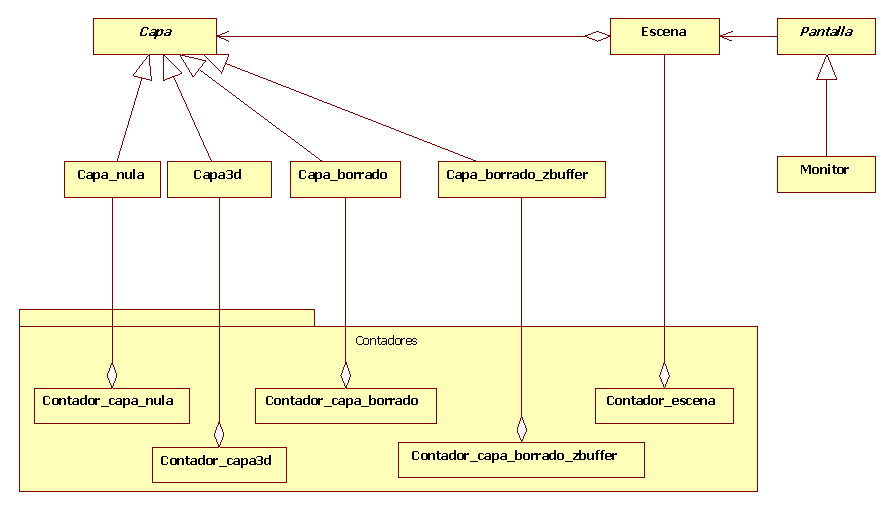
\includegraphics[width=14cm]{diagramas/analisis/render-clases.eps}

\caption{Diagrama de clases de an�lisis del nivel de pintado}
\end{figure}

\subsection{Capa}
Representa una capa de pintado en la escena. Cada capa pinta sobre las anteriores en la escena.
\begin{itemize}
\item \textbf{Responsabilidades:}
	\begin{itemize}
	\item Pintar lo que sea necesario sobre la escena.
	\end{itemize}
%\item \textbf{Relaciones:}
%\item \textbf{Atributos:}
%\item \textbf{M�todos:}
\end{itemize}

\subsection{Capa3d}
Representa una capa que pinta una escena 3D.
\begin{itemize}
\item \textbf{Responsabilidades:}
	\begin{itemize}
	\item Pintar la escena especificada.
	\end{itemize}
\item \textbf{Relaciones:}
	\begin{itemize}
	\item Es una especificaci�n de Capa.
	\item Depende de Objeto\_origen y C�mara.
	\end{itemize}
%\item \textbf{Atributos:}

%\item \textbf{M�todos:}
\end{itemize}

\subsection{Capa borrado}
Representa una capa que pinta toda la escena de un color uniforme.
\begin{itemize}
\item \textbf{Responsabilidades:}
	\begin{itemize}
	\item Pintar la escena del color indicado.
	\end{itemize}
\item \textbf{Relaciones:}
	\begin{itemize}
	\item Es una especificaci�n de Capa.
	\end{itemize}
\item \textbf{Atributos:}
	\begin{itemize}
	\item +color \newline
El color con el que se pintar� la escena.
	\end{itemize}
%\item \textbf{M�todos:}
\end{itemize}

\subsection{Capa borrado zbuffer}
Representa una capa que borra el buffer de profundidad.
\begin{itemize}
\item \textbf{Responsabilidades:}
	\begin{itemize}
	\item Pintar lo que sea necesario sobre la escena.
	\end{itemize}
\item \textbf{Relaciones:}
	\begin{itemize}
	\item Es una especificaci�n de Capa.
	\end{itemize}
%\item \textbf{Atributos:}
%\item \textbf{M�todos:}
\end{itemize}

\subsection{Escena}
Representa una escena compuesta por la aplicaci�n sucesiva de varias capas.
\begin{itemize}
\item \textbf{Responsabilidades:}
	\begin{itemize}
	\item Pintar las capas en el orden especificado.
	\end{itemize}
\item \textbf{Relaciones:}
	\begin{itemize}
	\item Agrega ordenadamente varias instancias de Capa.
	\end{itemize}

%\item \textbf{Atributos:}
%\item \textbf{M�todos:}
\end{itemize}

\subsection{Pantalla}
Representa una pantalla del ordenador, donde se proyecta una escena.
\begin{itemize}
\item \textbf{Responsabilidades:}
	\begin{itemize}
	\item Representar una pantalla, y asociar la escena correspondiente.
	\end{itemize}
\item \textbf{Relaciones:}
	\begin{itemize}
	\item Agrega ordenadamente varias instancias de Capa.
	\end{itemize}

\item \textbf{Atributos:}
	\begin{itemize}
	\item Ancho \newline
	El ancho de la pantalla.
	\item Alto \newline
	El alto de la pantalla.
	\end{itemize}
\item \textbf{M�todos:}
	\begin{itemize}
	\item Dimensiones \newline
	Devuelve las dimensiones de la pantalla (ancho y alto).
	\end{itemize}	
\end{itemize}

\subsection{Monitor}
Representa un monitor del ordenador.
\begin{itemize}
\item \textbf{Responsabilidades:}
	\begin{itemize}
	\item Representar un monitor del ordenador, y gestionar los accesos al sistema de ventanas si hubiera.
	\end{itemize}
\item \textbf{Relaciones:}
	\begin{itemize}
	\item Es una especificaci�n de Pantalla.
	\end{itemize}

\item \textbf{Atributos:}
	\begin{itemize}
	\item estado \newline
El estado del monitor, ya sea como ventana o pantalla completa en un gestor de ventanas, adem�s de su posici�n (primer o segundo plano).
	\end{itemize}
\item \textbf{M�todos:}
	\item +estado  \newline
	Getter.
	\item +cambiar\_modo \newline
	Cambia el modo de pantalla, o las dimensiones de la ventana.

\end{itemize}

\section{Subsistema de procesos}
Este subsistema proporciona una base para la implementaci�n de la l�gica del juego, basado en el modelo de procesos de un sistema operativo multitarea.


\begin{figure}[htp]
\centering
%\includegraphics[width=14cm]{analisis/propuesto/modelos_objeto/geometria/clases.eps}
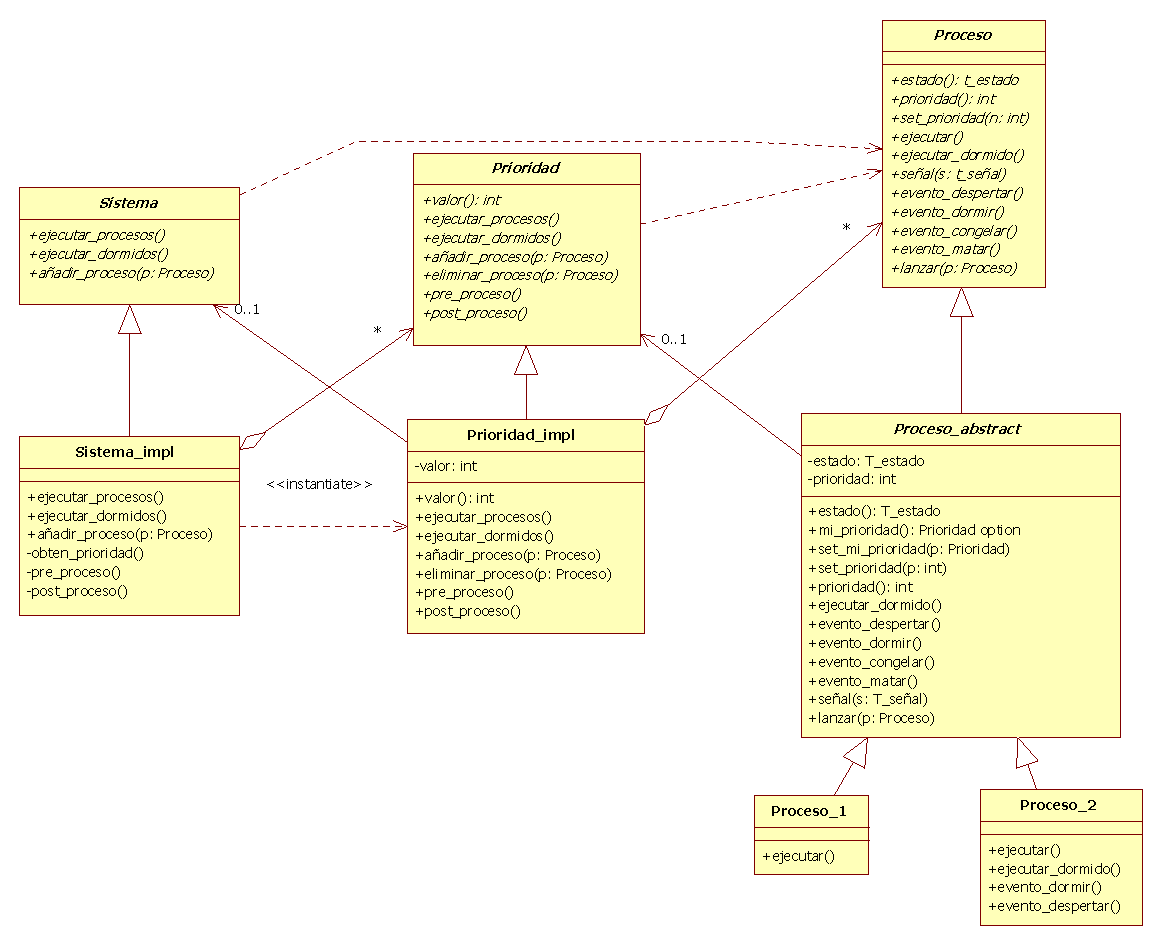
\includegraphics[width=14cm]{diagramas/analisis/procesos-clases.eps}
\caption{Diagrama de clases de an�lisis del subsistema de Procesos}
\end{figure}


\subsection{Sistema}
Representa un sistema de procesos.
\begin{itemize}
\item \textbf{Responsabilidades:}
	\begin{itemize}
	\item Almacenar y ordenar todos los procesos por prioridad.
	\item Dar una r�faga de CPU a cada proceso por orden de prioridad.
	\end{itemize}
\item \textbf{Relaciones:}
	\begin{itemize}
	\item Agrega Prioridad.
	\end{itemize}

%\item \textbf{Atributos:}
%	\begin{itemize}
%	\item estado \newline
%El estado del monitor, ya sea como ventana o pantalla completa en un gestor de ventanas, adem�s de su posici�n (primer o segundo plano).
%	\end{itemize}
\item \textbf{M�todos:}
	\item +ejecutar\_procesos  \newline
	Da una r�faga de CPU a los procesos despiertos.
	\item +ejecutar\_dormidos \newline
	Da una r�faga de CPU a los procesos dormidos.

\end{itemize}


\chapter{Modelos Din�micos}
\section{Objetos : establecer padre}
En el diagrama de secuencia se observa como se desarrolla la acci�n. El objeto \underline{m} pasa de ser descendiente de \underline{padre} a ser descendiente de \underline{nuevo\_padre}. Los pasos que ocurren son:
\begin{enumerate}
\item El usuario llama a cambiar\_padre(nuevo\_padre)
\end{enumerate}



\end{document}
